%\NeedsTeXFormat{LaTeX2e}
\documentclass[12pt]{article}

%%%% Seitenformat text={breite,h�he}
\usepackage[a4paper,top=3.0cm,left=3.0cm,right=2.7cm,bottom=2cm]{geometry}
\usepackage{url}

\setlength{\textheight}{240mm}

\setlength{\headsep}{10mm}


\usepackage[utf8]{inputenc}
\usepackage[T1]{fontenc}
\usepackage{lmodern}
\usepackage[ngerman]{babel}
\usepackage[pdftex]{graphicx}
\usepackage{wrapfig}

\usepackage{hyperref}






\newcommand{\mynote}[2]{\textbf{{#1}:}\textit{{#2}}}
\newcommand\timo[1]{\mynote{TIMO}{#1}}
\newcommand\manu[1]{\mynote{MANUEL}{#1}}


\begin{document}

\tableofcontents


\section{Grundlegendes}

\subsection{Semantic Lifting und asymmetrische Differenzen}
Auch geliftete Differenzen (Stand \cite{KeKT2011ASE} und \cite{Oh2012BA}) sind, 
obwohl die Semantic Change Sets ausgeführte Editieroperationen repräsentieren, 
immer noch symmetrische Differenzen.
Um geliftete Differenzen in asymmetrische (und damit ausführbare) Differenzen 
zu konvertieren, bedarf es noch zwei weiterer Analyseschritte:
\begin{enumerate}
 \item Erkennung sequentiell abhängiger Operationen
 \item Extraktion der aktuellen Aufrufparameter von Operationen
\end{enumerate}

Ferner muss eine gravierende Einschränkung des in \cite{KeKT2011ASE}
beschriebenen Konzepts behoben werden: Operationskontexte müssen
hier sowohl in A, als auch in B vollständig erhalten sein. Dies
ist eine zu restriktive Einschränkung. 
Ursache hierfür sind potentielle, sequentielle Abhängigkeiten der 
Editierregeln.


Wir führen neue konzeptuelle Enität in das Differenzmodell ein: \texttt{OperationInvocation}. 

\texttt{OperationInvocation} hat Multiplicity 0..1, da wir eine Konvertierung in asymmetrische Differenzen nicht zwangsläufig durchführen. Manchmal genügen einem vielleicht geliftete Differenzen (je nach Tool und Use Case). 

\texttt{changeSet} hat Multiplicity 0..1, da wir vielleicht die Changes und ChangeSets aus der Differenz wegwerfen (ganz am Ende), wenn wir ausschließlich an asymmetrischen Differenzen/Patches interessiert sind.

\begin{figure}[htb]
  \centering
  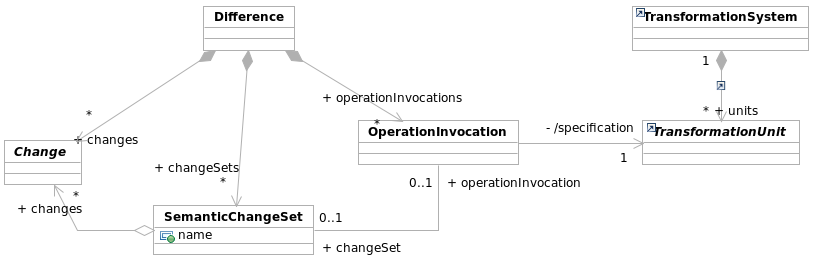
\includegraphics[width=1.0\textwidth]{img/OperationInvocation.png}
  \caption{OperationInvocation im Differenzmodell}
  \label{fig:OperationInvocation}
\end{figure}



\section{Analyse sequentieller Abhängigkeiten}

\subsection{Grenzen der Sequential-Recognition-Engine (SRE)}
Ein erster Schritt in Richtung asymmetrischer Differenzen ist 
die Sequential Recognition Engine \cite{Oh2012BA}, diese unterliegt jedoch 
Einschränkungen.

Der ursprüngliche Gedanke hinter der SRE war es, immer die Zwischenzustände zwischen Modell A und
Modell B zu berechnen. Wie sich herausstellt, funktioniert dies für das hinzufügen und entfernen von
Modell Elementen Problemlos, z.B. bei Verschiebungen von Modell Elementen ist aber nicht mehr
eindeutig klar wie der Zwischenzustand des Modells aussehen muss. Man kann sich überlegen, dass es
immer zwei mögliche Zustände gibt; vor dem Verschieben und nach dem Verschieben.

Dieses Problem und die Grenzen der SRE lassen sich begründen, wenn man den Algorithmus als eine
schrittweise Vereinigung von Modell A und Modell B betrachtet. Eine fehlerfrei Auflösung der
sequentiellen Abhängigkeiten ist immer dann möglich, wenn die Vereinigung von Modell A und Modell B
eindeutig ist.

Als nächstes stellt sich also die Frage, wann ist die Vereinigung nicht eindeutig. Allgemein lässt
sich sagen, dass die Vereinigung solange  eindeutig ist wie nur Elemente hinzugefügt oder entfernt
werden. Sobald bestehende Elemente verändert werden, gibt es keine eindeutige Vereinigung mehr. Die
Vereinigung ist also in folgenden Fällen nicht eindeutig zu bestimmen:

\begin{itemize}
  \item Bei allen Attribute-Value-Changes (AVC).
  \item Bei Veränderung von bestehenden Referenzen:
  \begin{itemize}
    \item Verschiebung von Objekten (\textit{move}); also der Veränderung einer
    Containment-Referenz.
    \item Immer wenn erforderliche (\textit{required}) Referenzen verändert werden.
    \item Aber auch wenn nicht erforderliche (bestehende) Referenzen verändert werden.
  \end{itemize}
\end{itemize}
\timo{AVC, move und ``target change'' von required (also Multiplicity 1) Referenzen sind mir
klar. Für nicht erforderliche Referenzen ist mir die Mehrdeutigkeit beim Vereinigen noch
unklar.}

\subsection{Bilden der Vereinigung}

Theoretisch können verschiedene Möglichkeiten gewählt werden um die Vereinigung der beiden Modelle
zu bilden. Wenn die oben beschriebenen Fälle vernachlässigt werden, sollte aber jede dieser
Möglichkeiten eine korrektes Lifting ermöglichen.

\begin{enumerate}
  \item \textbf{Schrittweise Vereinigung:} So wie im SRE Konzept beschrieben, werden immer die
  jeweils durch die Erkennungsregeln in einem Semantic-Change-Set zusammengefassten low-level
  Änderungen in Modell A oder Modell B eingefügt. Auf diese Art werden Schrittweise die
  sequenziell Abhängigen Editieroperationen erkannt.
  \item \textbf{Direkte Vereinigung:} Eine andere Möglichkeit wäre es, erst alle Teile die in
  Modell B vorkommen aber nicht in Modell A, in Modell A einzufügen und alle Teile die in Modell
  A vorkommen aber nicht in Modell B in Modell B einzufügen. Auf diese Weise wäre es möglich, in
  einem Schritt, sofort alle sequenziell Abhängigen Editieroperationen zu erkennen.
\end{enumerate}

Um Create-Use- und Removed-Used-Dependences zu erkennen, reicht es aus nur die Teile zu Vereinigen,
welche entweder hinzugefügt oder entfernt wurden. Alle Änderungen an bestehenden Teilen des
Modells können vernachlässigt werden. Alle anderen Abhängigkeiten werden so allerdings nicht
erkannt.

% \subsection{Mögliche sequentielle Abhängigkeiten}
% 
% \begin{itemize}
%   \item Create
%   \item Remove
%   \item Move/Change
%   \item AVC
% \end{itemize}
% 
% Create:
% 
% \begin{itemize}
%   \item Create $\rightarrow$ Create
%   \item Create $\rightarrow$ Remove
%   \item Create $\rightarrow$ Move/Change
%   \item Create $\rightarrow$ AVC
% \end{itemize}
% 
% Remove:
% 
% \begin{itemize}
%   \item Remove $\rightarrow$ Create
%   \item Remove $\rightarrow$ Remove
%   \item Remove $\rightarrow$ Move/Change
%   \item Remove $\rightarrow$ AVC
% \end{itemize}
% 
% Move/Change:
% 
% \begin{itemize}
%   \item Move/Change $\rightarrow$ Create
%   \item Move/Change $\rightarrow$ Remove
%   \item Move/Change $\rightarrow$ Move/Change
%   \item Move/Change $\rightarrow$ AVC
% \end{itemize}
% 
% AVC:
% 
% \begin{itemize}
%   \item AVC $\rightarrow$ Create
%   \item AVC $\rightarrow$ Remove
%   \item AVC $\rightarrow$ Move/Change
%   \item AVC $\rightarrow$ AVC
% \end{itemize}
% 
% Fraglich ob es wirklich jede möglich Kombination von sequentiellen Abhängigkeiten geben kann.

\subsection{Editierregel Analyse}

Im Sinne unserer Editierregeln treten sequentielle Abhängigkeiten immer dann auf, wenn ein
\texttt{<<preserve>>} Knoten zuvor durch eine andere Editieroperation erzeugt, gelöscht oder
verändert wurde. Eine ausführliche Betrachtung befindet sich im Dokument TODO.

Die \texttt{<<preserve>>} Knoten der Editierregel lassen sich als Kontext bzw. als
Precondition für die Editieroperation bezeichnen. Das Problem ist, dass Kontext und Preconditions
nicht immer sauber getrennt sind. Betrachtet man z.B. die Regel
\texttt{Move-EAttribute-To-Neighbour}, dann sind die beiden Klassen zwischen denen das Attribut
verschoben wird der Kontext für die Editieroperation. Die Referenz die zwischen den beiden Klassen
bestehen muss ist aber eigentlich als Precondition der Editieroperation anzusehen. Das gleiche gilt
eigentlich auch für alle (\texttt{<<preserve>>}/\texttt{<<delete>>}) Attributwerte die zum
anwenden der Editierregel einen bestimmten Wert haben müssen.

Vernachlässigt man sämtliche Preconditions der Editierregeln, so können sequentielle Abhängigkeiten
nur noch für den Kontext der Editierregel auftreten. Der Kontext der Editierregel lässt sich auch
relativ leicht von evtl. in der Editierregel enthaltenen Preconditions unterscheiden. Ein Kontext
Knoten muss mindestens eine ausgehende oder eingehende \texttt{<<delete>>} oder \texttt{<<create>>}
Kante haben oder mindestens eine "`Attribut setzt Operation"'. Alle \texttt{<<preserve>>} Kanten
wären dann ebenfalls als Preconditions zu behandeln.

Dieser Zusammenhang wird auch klar, wenn man bedenkt, dass die sequentiellen Abhängigkeiten (neben
den AVCs) nur durch die \texttt{<<preserve>>} Kanten in der Editierregel ausgelöst werden. Entfernt
man sämtliche \texttt{<<preserve>>} Kanten aus der Editierregel, so hängen die Precondition Knoten
in der Luft (und haben somit nur ein sehr begrenztes Nutzen).

Betrachtet man nun nochmal die potenziellen sequentiellen Abhängigkeiten der Editierregel, so
reduzieren sich diese wieder auf (die bereits besprochenen) Create-Use- und
Removed-Used-Dependences.

Entfernt man sämtliche Preconditions aus einer Editierregel, so könnte es bei manchen
Regeln passieren, dass diese dadurch in mehrere Teile zerfallen. Eben genau dann, wenn die einzelnen
Kontext Teile über \texttt{<<preserve>>} Knoten (und damit Preconditions) verbunden wurden. Ein
solcher Fall tritt z.B. bei der \textit{Pull-Up-Attribute} Regel auf. Hier zerfällt die Multi-Regel
in den \textit{Move-EAttribute} und den \textit{Delete-EAttribute} Teil. Klar wird damit auch, dass die
Preconditions nicht vollständig vernachlässigt werden können. Es wird aber im Zweifelsfall nur zu
viel erkannt. Fehlerhaft erkannte Editieroperationen müssen also später noch ausgeschlossen werden.

\subsection{Wann werden Preconditions benötigt?}

Wenn wir davon ausgehen, dass für Modell A und Modell B folgende Randbedingungen gelten, dann können
wir eine Aussage darüber treffen ob und wann Preconditions überhaupt benötigt werden.

\begin{enumerate}
  \item Beide Modelle erfüllen ihre technischen Constraints. 
  
  \begin{quote}
  	"`Verschiebt sich der Fokus vom Verändern eines gegebenen Graphen hin zum Erzeugen aller, aus
  	einem Startgraphen ableitbarer Graphen, wird von einer Graphgrammatik anstelle eines
  	Graphersetzungssystems und von Produktionen anstelle von Regeln gesprochen. Die Vereinigung der
  	beim systematischen Aufzählen entstehenden Graphen ist die Sprache der Graphgrammatik."'
    
    [http://de.wikipedia.org/wiki/Graphersetzung]
  \end{quote}
  
  Würde bedeuten, dass ein Modell A oder B in der Modellierungssprache liegt, wenn wir das jeweilige
  Modell nur durch atomare Einfüge-Operationen erzeugen können. Alle atomaren Einfüge-Operationen
  und AVC-Operationen wären also die Produktionen der Modellierungssprache.
  
  \item Wir haben eine vollständige atomare Regelbasis.
  
  \item Alle Korrespondenzen und die daraus resultierende Differenz wurde korrekt berechnet. Bei
  einer korrekten Differenz, sollte unter den in (1) und (2) gegebenen Bedingungen immer ein
  vollständiges Lifting existieren.
\end{enumerate}

Wir können also bei der Erfüllung dieser Randbedingungen und einer atomaren Regelbasis davon
ausgehen, dass ein \textbf{eindeutiges} Lifting der Differenz existiert. D.h. aber auch, dass die
Preconditions für atomare Regeln (tatsächlich) immer erfüllt sind, wenn die atomare Editierregel
erkannt wurde. Es gibt keine andere Möglichkeit die low-level Änderungen zu gruppieren.
Grundsätzlich wäre es also an dieser Stelle nicht nötig die Preconditions zu überprüfen.

Grundsätzlich müsste diese Annahme auch für komplexe Editieroperationen gelten, da diese sich im
Prinzip aus atomaren Editieroperationen zusammensetzen müssen. Damit gelten eben auch die selben
Preconditions wie für die jeweiligen atomaren Editieroperationen.

Als Gegenbeispiel für diese These könnte man nun die Editieroperation \textit{Pull-Up-Attribute}
betrachten. Hier muss es in jeder Subklasse mindestens ein entsprechendes Attribut geben. Diese
Preconditions ist eben nicht immer erfüllt, wenn Pull-Up-Attribut erkannt wurde. Der Grund für
dieses Problem ist aber, dass Pull-Up-Attribute eigentlich keine Editieroperation, nach den zuvor
beschriebenen Eigenschaften darstellt. Ein \textit{Pull-Up-Attribute} ist eigentlich gar keine reine
Editieropration sondern ein Refactoring. Es ist nicht möglich \textit{Pull-Up-Attribute} in atomare
Editierregeln und deren Preconditions zu zerlegen. Würde man die zuvor beschriebene Precondition
weglassen, dann wäre dies möglich und \textit{Pull-Up-Attribute} wäre immer noch eine korrekte
Editieroperation, da ja alle Constraints der Modellierungsprache trotzdem eingehalten werden. An
dieser Stelle könnte man folgende Unterscheidung zwischen Preconditions treffen.

\begin{itemize}
  \item \textbf{technische Preconditions:} Alle Preconditions die durch atomare Regeln vorgegeben
  werden, z.B. "`Jeder Klassenname darf nur einmal in einem Paket vorkommen."'.
  \item \textbf{semantische Preconditions:} Alles was über die technischen Preconditions hinaus
  geht, um wie z.B. bei \textit{Pull-Up-Attribute} eine bestimmte Semantik auf dem Modell zu
  erhalten/prüfen.
\end{itemize}

Folglich machen uns also hauptsächlich Editierregeln mit semantischen Preconditions Probleme, da
diese auf jeden Fall überprüft werden müssen.

Im Regel Fall kann man also davon ausgehen, dass Preconditions für erkannte atomare Editierregeln
erfüllt sind. Es wäre aber nicht unmöglich Regeln zu erzeugen wo dies nicht der Fall ist. Probleme
entstehen immer dann, wenn (nach Definition oben) Preconditions aus der Editierregel vernachlässigt
werden, welche eigentlich doch als Kontext benötigt werden. Zum Beispiel:

\begin{itemize}
  \item Eine atomare Regel zerfällt durch entfernen der \texttt{<<preserve>>} Precondition Knoten in
  mehrere Teile. Dadurch können, besonders dann wenn die Regel mehrfach angewendet wurde, die
  einzelnen Teile beim erkennen nicht mehr korrekt zugeordnet werden.
  \item Ein Attribut muss an mehreren Stellen im (erzeugten/entfernten) Graphen den gleichen Wert
  besitzen. Hier könnte es auch wieder Probleme bei mehrfach Anwendung der Regel geben.
\end{itemize}

Das solche Konstrukte in atomaren Regeln vorkommen, sollte aber eher eine Ausnahme darstellen.
Besonders deshalb, weil in beiden Fällen davon ausgegangen wird, dass durch die atomare Regel mehr
als eine Knoten im Graph erzeugt/entfernt wird. Was für atomare Regeln eher untypisch ist.

\subsection{Überprüfung der Preconditions}

Theoretisch müsste es ausreichen, dass entweder Modell A oder Modell B die Precondition der
Editierregel erfüllt. Auf diesem Gedanken beruht ja auch der Versuch die sequentiellen
Abhängigkeiten über eine Vereinigung von Modell A und Modell B aufzulösen. Das Problem ist, dass die
Precondition auch dann erfüllt ist, wenn der dafür nötige Zustand zwischen Modell A und Modell B
liegt. Durch eine Vereinigung der Modelle lassen sich aber, wie bereits erwähnt, nicht alle
möglichen Zwischenzustände darstellen.

Eine andere Möglichkeit wäre es die Precondition einmal auf Modell A und einmal auf Modell B zu
überprüfen. Konsequenterweise kann es dann sein, dass die Precondition auf den jeweiligen Modellen
nur zum Teil erfüllt wird. Eine Precondition müsste aber genau dann erfüllt sein, wenn die
Vereinigung der beiden teil Preconditions von Modell A und Modell B, wieder die vollständige
Precondition erfüllt.

% Aus Sicht unserer Erkennungsregeln würde das bedeuten, dass es zunächst einmal mindesten eine
% Abbildung für jedes Correspondence Pattern gibt. (Ausgehend von einer zuvor durchgeführten
% Vereinigung, bei der Änderungen nicht beachtet wurden s.o.) 
% 
% Problematisch wir es jetzt eigentlich erst, wenn die Preserve-Reference-Patterns überprüft werden.
% An dieser Stelle würde es ausreichen, wenn mindestens eine Lösung existiert, bei der wenigsten eine
% Seite jedes Preserve-Reference-Patterns auf den Arbeitsgraphen abgebildet werden kann.
% 
% Für Attribute gilt ähnliches. Es muss entweder ein Objekt in Modell A oder Modell B geben, auf
% welches das entsprechende Attribut besitzt.

% \subsection{(Preconditions für Einfüge-Editierregel)}
% 
% Wird durch eine Editierregel ein neuer Teil in ein Modell eingefügt, so kann es sein, dass für diese
% Einfüge-Editierregel bestimmte Preconditions bestehen. Gehen wir davon aus, dass die
% Editierregel eine atomare Editierregel ist, dann kann der Teil des Modells, welcher für die
% Precondition benötigt wird, (nach ausführen der Einfüge-Editierregel) nicht mehr nachträglich
% verändert/gelöscht werden, ohne dass das Modell inkonsistent wird. D.h. für uns, dass alle
% \texttt{<<preserve>>} Anteile einer reinen Einfüge-Editierregel, auch in Modell B noch vorhanden
% sein müssen. Folglich müssten in einem solchen Fall die Preconditions nur auf Modell B überprüft
% werden.


\subsection{Erweiterung des Differenzmodells}

Vorschlag:
\begin{figure}[htb]
  \centering
  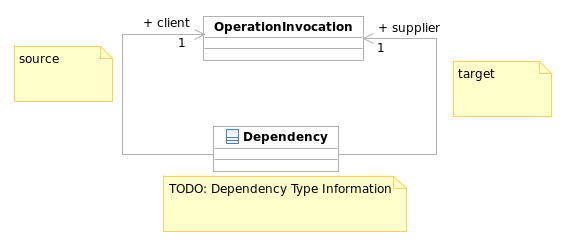
\includegraphics[width=0.8\textwidth]{img/Dependencies.png}
  \caption{Dependencies im Differenzmodell}
  \label{fig:Dependencies}
\end{figure}

\subsection{Ausblick}

Über das eigentliche Problem hinaus, könnte man bei der Precondition Prüfung auch feststellen,
welche Editieropration noch zusätzlich ausgeführt werden müsste, um die Precondition zu erfüllen.
Z.B., wenn für eine \texttt{Pull-Up-Attribute} Regel noch ein Attribut in einer Sub-Klasse fehlt,
könnte man dieses noch einfügen. Sozusagen die Differenz zwischen erfülltem Precondition Teil und
nicht erfülltem Precondition Teil.

\timo{Dies führt allerdings zur Erkennung von transienten Objekten. Diese wollen
wir bewusst aus unseren Betrachtungen ausklammern}


\section{Generierung der Erkennungsregeln}

Nehmen wir an, wir haben eine Folge von sequenziell abhängigen Editierregeln. Gehen wir zum Beispiel
davon aus, wir haben eine Klasse mit Namen \textit{C1} und einem Attribut \textit{A1}.
Nun erzeugen wir eine neue Klasse mit Namen \textit{C2} und verschieben nun \textit{A1} von
\textit{C1} nach \textit{C2}. Zum Schluss wird dann noch die Klasse \textit{C1} gelöscht. Um das
Beispiel einfach zu halten, gehen wir davon aus, dass \textit{C1} und \textit{C2} (auf Grund ihrer
Eigenschaften) in der Differenz nicht Korrespondieren. Sonst würde man die Transformation auf eine
Umbenennung (\textit{C1 $\to$ C2}) zurückführen. Daraus ergeben sich dann die sequenziell abhängigen
Editierregeln \textit{Create-Class} $\to$ \textit{Move-Attribute} $\to$ \textit{Delete-Class}.

\begin{figure}[htb]
  \centering
  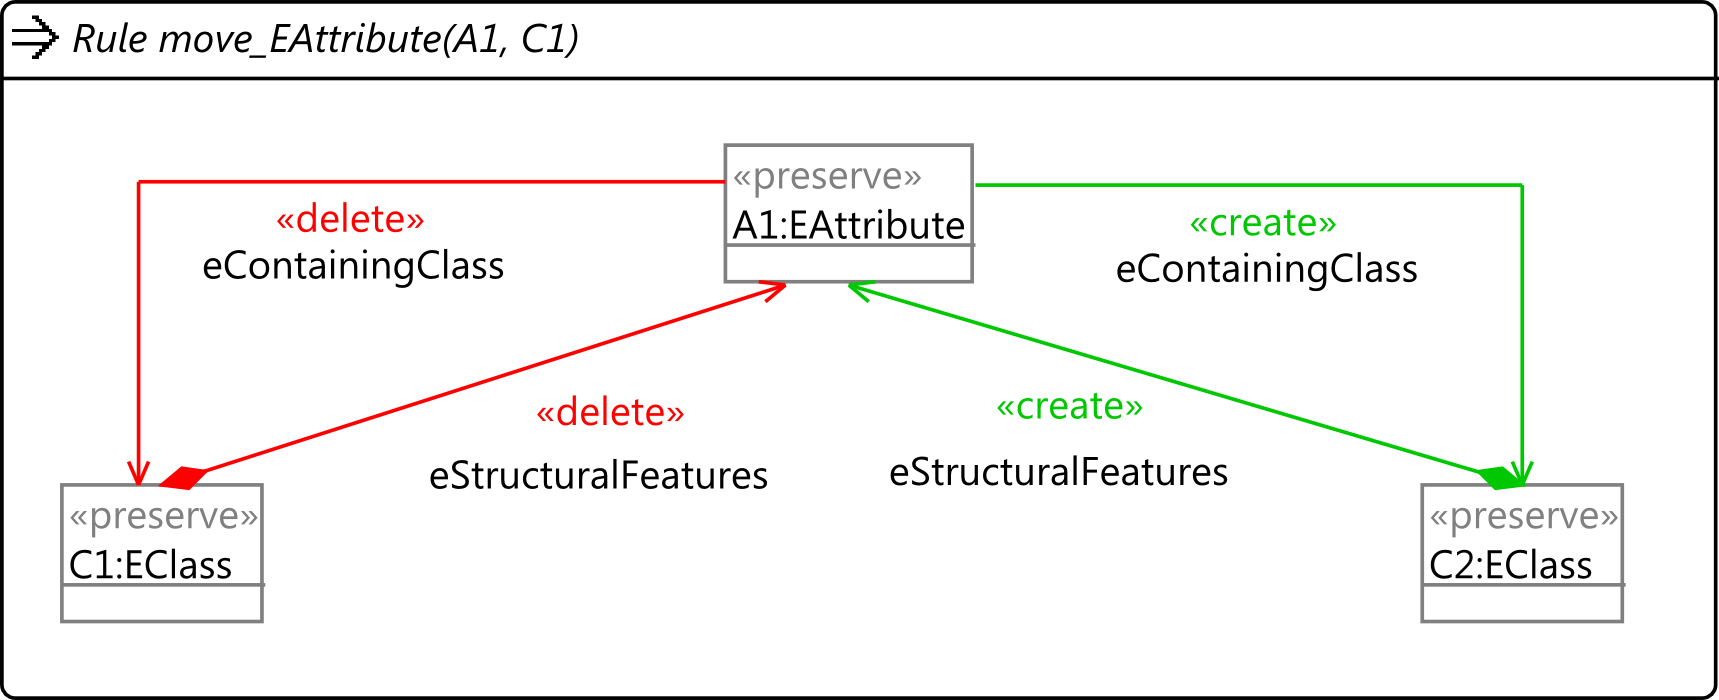
\includegraphics[width=1.0\textwidth]{img/move_eattribute_execute.png}
  \caption{Move-Attribute}
  \label{fig:Move-Attribute}
\end{figure}

Würden wir nun nach dem "`alten Konzept"' die jeweiligen Erkennungsregeln auf die Differenz
anwenden, so würden wir nur \textit{Create-Class} und \textit{Delete-Class} im ersten Durchlauf
erkennen. Für \textit{Move-Attribute} fehlen zunächst noch die Korrespondenzen für die Klassen
\textit{C1} und \textit{C2}. Unser Ziel ist es aber nun die Erkennungsregeln so anzupassen, dass
alle 3 Editieroperation in einem Durchlauf erkannt werden können. Dazu stellen wir zunächst die
umgekehrte Überlegung an. Wie können wir alle 3 Editieroperationen gleichzeitig auf Modell A
anwenden, um Modell B zu produzieren? - Wir müssten dazu einfach nur alle 3 Editieroperation zu
einer einzigen großen Editieroperation vereinigen. In diesem Fall würden die beiden
\texttt{<<preserve>>} Klassen der \textit{Move-Attribute} Editierregel jeweils durch die beiden
Editierregeln \textit{Create-Class} und \textit{Delete-Class} ersetzt.

Allgemein sollte es also möglich sein mehrere sequenziell abhängige Editierregeln zu einer einzigen
großen Editierregel zusammenzufassen. In diesem Fall sollte es aber auch möglich sein eine
Erkennungsregel zu generieren, welche in der Lage ist diese große Editierregel zu erkennen. Die
entscheidende Frage ist nun, können wir auch jede Editierregel für sich betrachtet, direkt durch
eine Erkennungsregel aus der Differenz wieder erkennen. 

An Hand dieses Beispiels wird klar, dass im Fall eines \texttt{<<preserve>>} Knoten in einer
Editierregel nicht zwangsläufig zu schlussfolgern ist, dass für diesen Knoten in der Erkennungsregel
eine Korrespondenz zweier Objekte existiert (vgl. Correspondence-Pattern). Es ist durchaus möglich,
dass ein Objekt nur in Modell A oder ein Objekt nur in Modell B vorkommt, welches dann für den
\texttt{<<preserve>>} Knoten der Editierregel erkannt werden muss. Das Gute ist, ob ein Objekt in
Modell A oder Modell B oder beiden vorkommen muss, lässt sich direkt aus der Editierregel ablesen.
Im Fall unserer \textit{Move-Attribute} Regel kann es keine weiteren sequentiellen Abhängigkeiten
geben, als: 

\begin{itemize}
  \item Die Klasse \textit{C1} kann entweder schon existieren oder später gelöscht werden. D.h. aber aber
  auch, dass sie in jedem Fall in Modell A existiert. Man könnte auch die Gegenprobe machen und
  versuchen, den \texttt{<<preserve>>} Knoten \textit{C1} in der \textit{Move-Attribute} Regel durch
  einen \texttt{<<create>>} Knoten zu ersetzen. Dies ist aber nicht möglich aufgrund der ausgehenden
  \texttt{<<delete>>} Kanten. Also brauchen wir für \textit{C1} auch in der Erkennungsregel kein
  vollständiges Correspondence-Pattern zu generieren. Es reicht aus nur den Modell A Knoten zu
  erzeugen.

  \item Für \textit{C2} gilt das umgekehrte, die Klasse kann entweder schon existieren oder sie wird
  zunächst neu erzeugt. Was bedeutet, dass sie in jedem Fall in Modell B vorhanden sein muss. Analog
  reicht es also hier aus das Correspondence-Pattern auf den Modell B Knoten einzuschränken.

  \item Das Attribut \textit{A1} muss auf jeden Fall sowohl in Modell A als auch in Modell B
  vorkommen. Dies wir auch in der Editierregel klar. Es ist, auf Grund der ausgehenden
  \texttt{<<create>>} und \texttt{<<delete>>} Kanten, nicht möglich den \texttt{<<preserve>>} Knoten
  \textit{A1} durch einen \texttt{<<create>>} Knoten oder \texttt{<<delete>>} Knoten zu ersetzen. In
  diesem Fall wird auch ein vollständiges Correspondence-Pattern benötigt.
\end{itemize}

\subsection{Algorithmus}

Der Erkennungsregel Generierungsalgorithmus muss also für das Correspondence-Pattern (CP) und daraus
resultierend auch für das Preserve-Reference-Pattern (PRP) angepasst werden. Wir betrachten also
folgende Möglichkeiten, die in einer Editierregel auftreten können:

\begin{enumerate}
  \item[CP1:] \texttt{<<preserve>>} Knoten mit ein- oder ausgehenden \texttt{<<delete>>} Kanten.
  
  $\Rightarrow$ Nur Modell A Knoten generieren.

  \item[CP2:] \texttt{<<preserve>>} Knoten mit ein- oder ausgehenden \texttt{<<create>>} Kanten.
  
  $\Rightarrow$ Nur Modell B Knoten generieren.

  \item[CP3:] \texttt{<<preserve>>} Knoten mit ein- oder ausgehenden \texttt{<<create>>} und
  \texttt{<<delete>>} Kanten.
  
  $\Rightarrow$ Vollständiges CP generieren.
\end{enumerate}

Für das reine Correspondence-Pattern reichen diese Fälle aus. Für \texttt{<<preserve>>} Kanten in
der Editierregel, wird das Ganze noch etwas komplizierter. Zunächst einmal können
\texttt{<<preserve>>} Kanten nur zwischen \texttt{<<preserve>>} Knoten existieren.

\begin{enumerate}
  \item[PRP1:] \texttt{<<preserve>>} Kante zwischen \textit{CP1} und \textit{CP1}.

  $\Rightarrow$ PRP wird nur zwischen Modell A Knoten generieren.

  \item[PRP2:] \texttt{<<preserve>>} Kante zwischen \textit{CP2} und \textit{CP2}.
  
  $\Rightarrow$ PRP wird nur zwischen Modell B Knoten generieren.
  
  \item[PRP3:] \texttt{<<preserve>>} Kante zwischen \textit{CP3} und \textit{CP3}.

  $\Rightarrow$ PRP wird zwischen Modell A und Modell B Knoten generieren.

  \item[PRP4:] \texttt{<<preserve>>} Kante zwischen \textit{CP1} und \textit{CP3}.
  
  $\Rightarrow$ PRP wird nur zwischen Modell A Knoten generieren.
  
  \item[PRP5:] \texttt{<<preserve>>} Kante zwischen \textit{CP2} und \textit{CP3}.
  
  $\Rightarrow$ PRP wird nur zwischen Modell B Knoten generieren.
  
  \item[PRP6:] \texttt{<<preserve>>} Kante zwischen \textit{CP1} und \textit{CP2}.
  
   $\Rightarrow$ Die bisherigen Fälle des PRP sind eigentlich Trivial, da immer sofort klar ist auf
   welcher Seite das PRP überhaupt generiert werden kann. In diesem Fall haben wir zunächst das
   Problem, dass wir nur einen Modell A und nur einen Modell B Knoten haben. Zwischen diesen beiden
   Knoten können wir aber kein PRP einfügen...
   
   \timo{Richtig, folgende Lösungsmöglichkeiten hatten wir diskutiert:}
   \begin{itemize}
    \item[A] \texttt{<<preserve>>} Kante aus der Erkennungsregel heraus lassen. 
    Dadurch werden keine Editieroperationen ``verpasst'' allerdings u.U. zu viele gematched,
    da eine positive Precondition nicht erfüllt ist.
    Dem wird bei der Abhängigkeitsanalyse entgegen gewirkt, da wir hier die Precondition
    explizit prüfen.
    \item[B] Erweitern der betroffenen \textit{CP1} und \textit{CP2}, jeweils zu \textit{CP3}.
    Wir verpassen hier u.U. die Erkennung einiger Editieroperationen, da der zur Anwendung
    notwendige Kontext nur temporär vorhanden war (aber weder in A noch in B vollständig vorhanden).
    Solange nachher wieder alles in die Erkennung atomarer Operationen zerfällt kein Problem.
    Intuitiv würde ich sagen es ist so, eine Argumentation dafür fällt schwer?
    \item[C] Man braüchte eine Art logische Verknüpfung auf Multi-Anteilen einer
    AmalgamationUnit, dann könnte man eine Erkennungsregel formulieren.
   \end{itemize}
   \timo{Ich tendiere ganz klar zu Lösung A}
   
\end{enumerate}

Den Fall \textit{PRP6} könnte man in Beispiel von oben, erzeugen in dem man in der
\textit{Move-Attribute} Regel zwischen \textit{C1} und \textit{C2} eine \texttt{<<preserve>>} Kante
einfügt, z.B. eine \textit{eSuperTypes}...

\begin{quote}Nochmal besprechen: Positive Preconditions können immer auf Modell B
überprüft werden. Da Positive Preconditions nach anwenden der Regel nicht mehr verändert
werden dürfen.\end{quote}
\timo{Man könnte so argumentieren. Allerdings gehen uns hier die temporär erfüllten Preconditions
und damit auch die Erkennung der jeweiligen Operationen durch die Lappen. 
Da wir ohnehin die Preconditions bei der Abhängigkeitsanalyse nochmals überprüfen müssen
(s. Lösungsvariante A oben, s. \ref{}), würde ich zunächst auf diese Einschränkung verzichten.
Letzten Endes ist dies eine Geschmacksfrage.
In der finalen Lösung sollten wir das vermutlich über einen Konfigurationsparameter steuern,
um verschiedenen Benutzerpräferenzen Rechnung zu tragen}

\begin{quote}TODO: Attribute?\end{quote}


\section{Operationserkennung}

RuleBase atomicR = ...   // Erkennungsregeln atomarer Operationen
RuleBase complexR = ...  // Erkennungsregeln komplexer Operationen

function operationRecognition(Difference d){
  recognizeAtomics(d);
  recognizeComplex(d);
}

function recognizeAtomics(Difference d){  
  applyRecognitionRules(atomicR); // Parallele Anwendung der atom. Erk.Regeln
  // kein postprocessing nötig!
  atomicDependencyAnalysis(); // 
}

function recognizeComplex(Difference d){

}


atomicDependencyAnalysis

Idee: transformiere Modell A schrittweise in Modell B. In jedem
Schritt sind 1..n Editierregeln anwendbar. Eben genau jene,
welche untereinander keine sequentiellen Abhängigkeiten 
besitzen.

Herausforderung: Wie kann man aus den gegebenen Informationen
(bislang nur ein SemanticChangeSet für das wir wissen, welche
Editieroperation es repräsentiert) eine Editierregel überhaupt
auf A (bzw. A') anwenden? 

Lösungsansatz: Wir ändern applyRecognitionRules() dahingehend,
dass wir uns die Matches der Erkennungsregeln merken. Haben
wir nun zusätzlich die Traces aus der Transformation editR2RecognitionR,
so können wir den Kontext für eine Editierregel wieder
rekonstruieren. Aber Achtung: der Kontext der Editierregel
muss nicht vollständig in der Erkennungsregel enthalten
sein (s. Abschnitt \ref{}).

Die Rekonstruktion des Kontextes ist jedoch nur möglich,
wenn dieser bereits existiert. Für direkt auf A anwendbare
Editierregeln (keine seq. Abhängigkeiten zu Vorgängern) ist
dies immer erfüllt.


\section{Parameter Retrieval}

\subsection{Arten von Operationsparametern}
Konzeptuell unterscheiden wir folgende Arten/Kategorien von Parametern: Objekt-Parameter und Value-Parameter


\subsubsection{Objekt-Parameter}
Parameter zur Identifikation von Objekten:

\begin{itemize}
 
 \item ``Echte'' \textbf{Objektreferenzen}: Hier werden einer Henshin-Rule direkt EObjects übergeben. Wenn ich mich richtig erinnere, 	gilt per Konvention folgendes: Entspricht der Parametername der ID eines Knotens einer Regel (normalerweise ist diese ID Schall und Rauch), so wird das übergebene Objekt per Prematch direkt gesetzt.
 
 \item \textbf{Symbolische Referenzen}: Technisch ist dies nur ein Value-Parameter (s. unten). Es wird einfach ein Attributwert (z.B. Name) übergeben, welcher ein Objekt eindeutig identifiziert. So z.B. beim Ecore-Refactoring move\_eattribute\_to\_neighbour. Konzeptuell handelt es sich jedoch um einen Objekt-Parameter.
 
\timo{Man kann diese Art der symbolischen Objektreferenzierung gerade bei EMF-Refactor sehr oft beobachten. Die frage ist nun, ob dies bei EMF-Refactor nur ein Workaround ist. Unter Umständen sollten wir symbolische Objektreferenzen vermeiden, da wir sie nicht von Value-Parametern unterscheiden können. Ist eine technische Frage, müssen wir aber klären}

\end{itemize}




\subsubsection{Value-Parameter} 
Hier werden einfache Literale (Strings, Integer etc.) übergeben

\begin{itemize}
  \item \textbf{Preconditions}
  \item Modifikation von Attributwerten
    \begin{itemize}
      \item \textbf{SET-Parameter}: Einfaches Setzen von Attributwerten
      \item \textbf{Funktionsparameter} von Berechnungen
    \end{itemize}
\end{itemize}


\paragraph{Preconditions}
\begin{itemize}
 \item Beispiel: PullUpAttribute. ``Alle Klassenattribute müssen den gleichen Namen haben''
 \item In der Editierregel ist hier nur die LHS vorhanden (oder LHS und RHS sind gleich)
 
\end{itemize}



\subsection{Erweiterung des Differenzmodells}

\begin{figure}[htb]
  \centering
  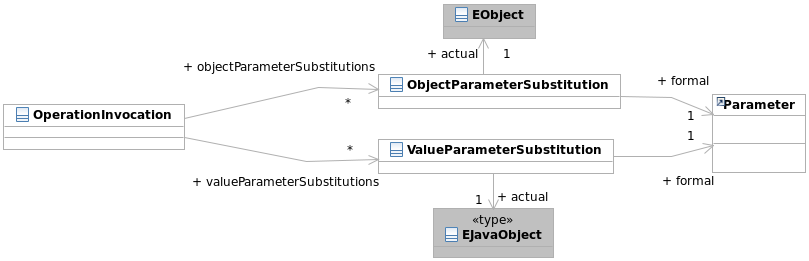
\includegraphics[width=1.2\textwidth]{img/Parameter.png}
  \caption{Parameter-Retrieval im Differenzmodell}
  \label{fig:Parameter}
\end{figure}






%%%%%%%%%%%%%%%%%%%%%%%%%%%%%%%%%%%%%%%%%%%%%%%%%%%%%%%%%%%%%%%%5

\begin{thebibliography}{xx}

\bibitem {KeKT2011ASE} {Kehrer, T.; Kelter, U.;
Taentzer, G.: A Rule-Based Approach to the Semantic
Lifting of Model Differences in the Context of Model
Versioning; p.163-172 in: Proc. 26th IEEE/ACM Intl. Conf.
Automated Software Engineering (ASE 2011); ACM; 2011}

\bibitem {Oh2012BA} {Ohrndorf, M.: 
Automatisierte Erzeugung von Transformationsregeln zur 
Optimierung von Modelldifferenzen ;
Bachelorarbeit; Univesität Siegen; 2012}

\end{thebibliography}

\end{document}















